\chapter{Моделирование одиночной РЛС}
\label{cha:analysis}

В данном разделе были рассмотрены пункты, связанные с моделированием случая одиночно расположенной радиолокационной станции. На рис. \ref{fig:RLS_1_dist} представлена зависимость вероятности правильного обнаружения от дальности до объекта.

\begin{figure}
    \centering
    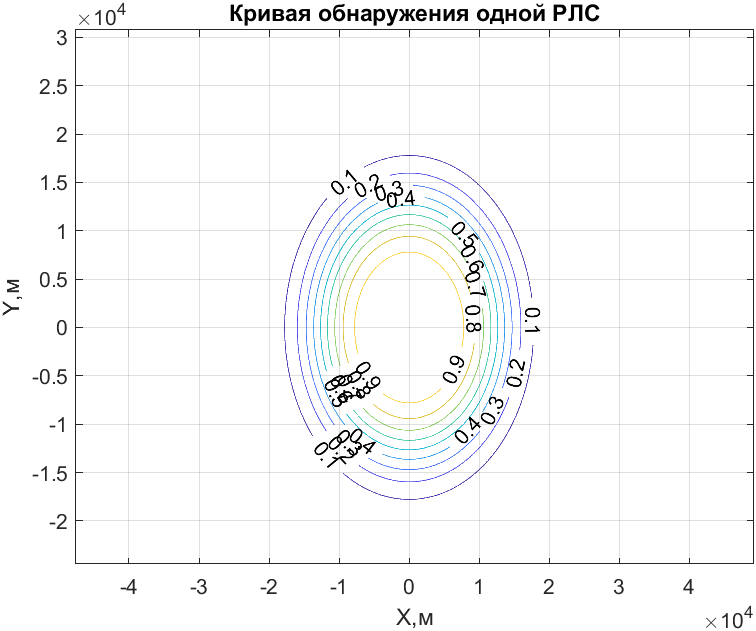
\includegraphics{figures/SingleRLS.png}
    \caption{Зависимость вероятности обнаружения от дальности для одиночно расположенной РЛС}
    \label{fig:RLS_1_dist}
\end{figure}
